% GNUPLOT: LaTeX picture with Postscript
\documentclass{minimal}
% Set font size
\makeatletter
\def\@ptsize{1}
\InputIfFileExists{size11.clo}{}{%
   \GenericError{(gnuplot) \space\space\space\@spaces}{%
      Gnuplot Error: File `size11.clo' not found! Could not set font size%
   }{See the gnuplot documentation for explanation.%
   }{For using a font size a file `size<fontsize>.clo' has to exist.
        Falling back ^^Jto default fontsize 10pt.}%
  \def\@ptsize{0}
  \input{size10.clo}%
}%
\makeatother
% Load packages
\usepackage{calc}
\usepackage{graphicx}
\usepackage{color}
\usepackage{transparent}
\makeatletter
% Select an appropriate default driver (from TeXLive graphics.cfg)
\begingroup
  \chardef\x=0 %
  % check pdfTeX
  \@ifundefined{pdfoutput}{}{%
    \ifcase\pdfoutput
    \else
      \chardef\x=1 %
    \fi
  }%
  % check VTeX
  \@ifundefined{OpMode}{}{%
    \chardef\x=2 %
  }%
\expandafter\endgroup
\ifcase\x
  % default case
  \PassOptionsToPackage{dvips}{geometry}
\or
  % pdfTeX is running in pdf mode
  \PassOptionsToPackage{pdftex}{geometry}
\else
  % VTeX is running
  \PassOptionsToPackage{vtex}{geometry}
\fi
\makeatother
% Set papersize
\usepackage[papersize={566.00bp,1700.00bp},text={566.00bp,1700.00bp}]{geometry}
% No page numbers and no paragraph indentation
\pagestyle{empty}
\setlength{\parindent}{0bp}%
% Load configuration file
\InputIfFileExists{gnuplot.cfg}{%
  \typeout{Using configuration file gnuplot.cfg}%
}{%
 \typeout{No configuration file gnuplot.cfg found.}%
}%
%
\begin{document}
\begingroup
  \makeatletter
  \providecommand\color[2][]{%
    \GenericError{(gnuplot) \space\space\space\@spaces}{%
      Package color not loaded in conjunction with
      terminal option `colourtext'%
    }{See the gnuplot documentation for explanation.%
    }{Either use 'blacktext' in gnuplot or load the package
      color.sty in LaTeX.}%
    \renewcommand\color[2][]{}%
  }%
  \providecommand\includegraphics[2][]{%
    \GenericError{(gnuplot) \space\space\space\@spaces}{%
      Package graphicx or graphics not loaded%
    }{See the gnuplot documentation for explanation.%
    }{The gnuplot epslatex terminal needs graphicx.sty or graphics.sty.}%
    \renewcommand\includegraphics[2][]{}%
  }%
  \providecommand\rotatebox[2]{#2}%
  \@ifundefined{ifGPcolor}{%
    \newif\ifGPcolor
    \GPcolortrue
  }{}%
  \@ifundefined{ifGPblacktext}{%
    \newif\ifGPblacktext
    \GPblacktextfalse
  }{}%
  % define a \g@addto@macro without @ in the name:
  \let\gplgaddtomacro\g@addto@macro
  % define empty templates for all commands taking text:
  \gdef\gplbacktext{}%
  \gdef\gplfronttext{}%
  \makeatother
  \ifGPblacktext
    % no textcolor at all
    \def\colorrgb#1{}%
    \def\colorgray#1{}%
  \else
    % gray or color?
    \ifGPcolor
      \def\colorrgb#1{\color[rgb]{#1}}%
      \def\colorgray#1{\color[gray]{#1}}%
      \expandafter\def\csname LTw\endcsname{\color{white}}%
      \expandafter\def\csname LTb\endcsname{\color{black}}%
      \expandafter\def\csname LTa\endcsname{\color{black}}%
      \expandafter\def\csname LT0\endcsname{\color[rgb]{1,0,0}}%
      \expandafter\def\csname LT1\endcsname{\color[rgb]{0,1,0}}%
      \expandafter\def\csname LT2\endcsname{\color[rgb]{0,0,1}}%
      \expandafter\def\csname LT3\endcsname{\color[rgb]{1,0,1}}%
      \expandafter\def\csname LT4\endcsname{\color[rgb]{0,1,1}}%
      \expandafter\def\csname LT5\endcsname{\color[rgb]{1,1,0}}%
      \expandafter\def\csname LT6\endcsname{\color[rgb]{0,0,0}}%
      \expandafter\def\csname LT7\endcsname{\color[rgb]{1,0.3,0}}%
      \expandafter\def\csname LT8\endcsname{\color[rgb]{0.5,0.5,0.5}}%
    \else
      % gray
      \def\colorrgb#1{\color{black}}%
      \def\colorgray#1{\color[gray]{#1}}%
      \expandafter\def\csname LTw\endcsname{\color{white}}%
      \expandafter\def\csname LTb\endcsname{\color{black}}%
      \expandafter\def\csname LTa\endcsname{\color{black}}%
      \expandafter\def\csname LT0\endcsname{\color{black}}%
      \expandafter\def\csname LT1\endcsname{\color{black}}%
      \expandafter\def\csname LT2\endcsname{\color{black}}%
      \expandafter\def\csname LT3\endcsname{\color{black}}%
      \expandafter\def\csname LT4\endcsname{\color{black}}%
      \expandafter\def\csname LT5\endcsname{\color{black}}%
      \expandafter\def\csname LT6\endcsname{\color{black}}%
      \expandafter\def\csname LT7\endcsname{\color{black}}%
      \expandafter\def\csname LT8\endcsname{\color{black}}%
    \fi
  \fi
    \setlength{\unitlength}{0.0500bp}%
    \ifx\gptboxheight\undefined%
      \newlength{\gptboxheight}%
      \newlength{\gptboxwidth}%
      \newsavebox{\gptboxtext}%
    \fi%
    \setlength{\fboxrule}{0.5pt}%
    \setlength{\fboxsep}{1pt}%
\begin{picture}(11320.00,34000.00)%
    \gplgaddtomacro\gplbacktext{%
      \csname LTb\endcsname%%
      \put(1256,26265){\makebox(0,0)[r]{\strut{}$0$}}%
      \csname LTb\endcsname%%
      \put(1256,27608){\makebox(0,0)[r]{\strut{}$500$}}%
      \csname LTb\endcsname%%
      \put(1256,28951){\makebox(0,0)[r]{\strut{}$1000$}}%
      \csname LTb\endcsname%%
      \put(1256,30293){\makebox(0,0)[r]{\strut{}$1500$}}%
      \csname LTb\endcsname%%
      \put(1256,31636){\makebox(0,0)[r]{\strut{}$2000$}}%
      \csname LTb\endcsname%%
      \put(1256,32979){\makebox(0,0)[r]{\strut{}$2500$}}%
      \csname LTb\endcsname%%
      \put(1358,26079){\makebox(0,0){\strut{}$-4$}}%
      \csname LTb\endcsname%%
      \put(2532,26079){\makebox(0,0){\strut{}$-3$}}%
      \csname LTb\endcsname%%
      \put(3707,26079){\makebox(0,0){\strut{}$-2$}}%
      \csname LTb\endcsname%%
      \put(4881,26079){\makebox(0,0){\strut{}$-1$}}%
      \csname LTb\endcsname%%
      \put(6056,26079){\makebox(0,0){\strut{}$0$}}%
      \csname LTb\endcsname%%
      \put(7230,26079){\makebox(0,0){\strut{}$1$}}%
      \csname LTb\endcsname%%
      \put(8404,26079){\makebox(0,0){\strut{}$2$}}%
      \csname LTb\endcsname%%
      \put(9579,26079){\makebox(0,0){\strut{}$3$}}%
      \csname LTb\endcsname%%
      \put(10753,26079){\makebox(0,0){\strut{}$4$}}%
    }%
    \gplgaddtomacro\gplfronttext{%
      \csname LTb\endcsname%%
      \put(458,29622){\rotatebox{-270}{\makebox(0,0){\strut{}\Huge Frequency}}}%
      \csname LTb\endcsname%%
      \put(6055,25614){\makebox(0,0){\strut{}\Huge$x$}}%
      \csname LTb\endcsname%%
      \put(9965,32812){\makebox(0,0)[r]{\strut{}Simulation}}%
      \csname LTb\endcsname%%
      \put(9965,32626){\makebox(0,0)[r]{\strut{}Theory}}%
      \csname LTb\endcsname%%
      \put(1640,32442){\makebox(0,0)[l]{\strut{}\huge$\mu=0,\sigma=1$}}%
    }%
    \gplgaddtomacro\gplbacktext{%
      \csname LTb\endcsname%%
      \put(1256,17850){\makebox(0,0)[r]{\strut{}$0$}}%
      \csname LTb\endcsname%%
      \put(1256,18809){\makebox(0,0)[r]{\strut{}$2000$}}%
      \csname LTb\endcsname%%
      \put(1256,19768){\makebox(0,0)[r]{\strut{}$4000$}}%
      \csname LTb\endcsname%%
      \put(1256,20727){\makebox(0,0)[r]{\strut{}$6000$}}%
      \csname LTb\endcsname%%
      \put(1256,21687){\makebox(0,0)[r]{\strut{}$8000$}}%
      \csname LTb\endcsname%%
      \put(1256,22646){\makebox(0,0)[r]{\strut{}$10000$}}%
      \csname LTb\endcsname%%
      \put(1256,23605){\makebox(0,0)[r]{\strut{}$12000$}}%
      \csname LTb\endcsname%%
      \put(1256,24564){\makebox(0,0)[r]{\strut{}$14000$}}%
      \csname LTb\endcsname%%
      \put(1358,17664){\makebox(0,0){\strut{}$-10$}}%
      \csname LTb\endcsname%%
      \put(2298,17664){\makebox(0,0){\strut{}$-8$}}%
      \csname LTb\endcsname%%
      \put(3237,17664){\makebox(0,0){\strut{}$-6$}}%
      \csname LTb\endcsname%%
      \put(4177,17664){\makebox(0,0){\strut{}$-4$}}%
      \csname LTb\endcsname%%
      \put(5116,17664){\makebox(0,0){\strut{}$-2$}}%
      \csname LTb\endcsname%%
      \put(6056,17664){\makebox(0,0){\strut{}$0$}}%
      \csname LTb\endcsname%%
      \put(6995,17664){\makebox(0,0){\strut{}$2$}}%
      \csname LTb\endcsname%%
      \put(7935,17664){\makebox(0,0){\strut{}$4$}}%
      \csname LTb\endcsname%%
      \put(8874,17664){\makebox(0,0){\strut{}$6$}}%
      \csname LTb\endcsname%%
      \put(9814,17664){\makebox(0,0){\strut{}$8$}}%
      \csname LTb\endcsname%%
      \put(10753,17664){\makebox(0,0){\strut{}$10$}}%
    }%
    \gplgaddtomacro\gplfronttext{%
      \csname LTb\endcsname%%
      \put(356,21207){\rotatebox{-270}{\makebox(0,0){\strut{}\Huge Frequency}}}%
      \csname LTb\endcsname%%
      \put(6055,17199){\makebox(0,0){\strut{}\Huge$x$}}%
      \csname LTb\endcsname%%
      \put(9965,24397){\makebox(0,0)[r]{\strut{}Simulation}}%
      \csname LTb\endcsname%%
      \put(9965,24211){\makebox(0,0)[r]{\strut{}Theory}}%
      \csname LTb\endcsname%%
      \put(1640,24027){\makebox(0,0)[l]{\strut{}\huge$\mu=\pm2,\sigma=1$}}%
    }%
    \gplgaddtomacro\gplbacktext{%
      \csname LTb\endcsname%%
      \put(1256,9434){\makebox(0,0)[r]{\strut{}$0$}}%
      \csname LTb\endcsname%%
      \put(1256,10106){\makebox(0,0)[r]{\strut{}$1000$}}%
      \csname LTb\endcsname%%
      \put(1256,10777){\makebox(0,0)[r]{\strut{}$2000$}}%
      \csname LTb\endcsname%%
      \put(1256,11449){\makebox(0,0)[r]{\strut{}$3000$}}%
      \csname LTb\endcsname%%
      \put(1256,12120){\makebox(0,0)[r]{\strut{}$4000$}}%
      \csname LTb\endcsname%%
      \put(1256,12792){\makebox(0,0)[r]{\strut{}$5000$}}%
      \csname LTb\endcsname%%
      \put(1256,13463){\makebox(0,0)[r]{\strut{}$6000$}}%
      \csname LTb\endcsname%%
      \put(1256,14135){\makebox(0,0)[r]{\strut{}$7000$}}%
      \csname LTb\endcsname%%
      \put(1256,14806){\makebox(0,0)[r]{\strut{}$8000$}}%
      \csname LTb\endcsname%%
      \put(1256,15478){\makebox(0,0)[r]{\strut{}$9000$}}%
      \csname LTb\endcsname%%
      \put(1256,16149){\makebox(0,0)[r]{\strut{}$10000$}}%
      \csname LTb\endcsname%%
      \put(1358,9248){\makebox(0,0){\strut{}$-10$}}%
      \csname LTb\endcsname%%
      \put(2298,9248){\makebox(0,0){\strut{}$-8$}}%
      \csname LTb\endcsname%%
      \put(3237,9248){\makebox(0,0){\strut{}$-6$}}%
      \csname LTb\endcsname%%
      \put(4177,9248){\makebox(0,0){\strut{}$-4$}}%
      \csname LTb\endcsname%%
      \put(5116,9248){\makebox(0,0){\strut{}$-2$}}%
      \csname LTb\endcsname%%
      \put(6056,9248){\makebox(0,0){\strut{}$0$}}%
      \csname LTb\endcsname%%
      \put(6995,9248){\makebox(0,0){\strut{}$2$}}%
      \csname LTb\endcsname%%
      \put(7935,9248){\makebox(0,0){\strut{}$4$}}%
      \csname LTb\endcsname%%
      \put(8874,9248){\makebox(0,0){\strut{}$6$}}%
      \csname LTb\endcsname%%
      \put(9814,9248){\makebox(0,0){\strut{}$8$}}%
      \csname LTb\endcsname%%
      \put(10753,9248){\makebox(0,0){\strut{}$10$}}%
    }%
    \gplgaddtomacro\gplfronttext{%
      \csname LTb\endcsname%%
      \put(356,12791){\rotatebox{-270}{\makebox(0,0){\strut{}\Huge Frequency}}}%
      \csname LTb\endcsname%%
      \put(6055,8783){\makebox(0,0){\strut{}\Huge$x$}}%
      \csname LTb\endcsname%%
      \put(9965,15982){\makebox(0,0)[r]{\strut{}Simulation}}%
      \csname LTb\endcsname%%
      \put(9965,15796){\makebox(0,0)[r]{\strut{}Theory}}%
      \csname LTb\endcsname%%
      \put(1640,15612){\makebox(0,0)[l]{\strut{}\huge$\mu=\left\{-5,0,5\right\}$}}%
      \csname LTb\endcsname%%
      \put(1640,14940){\makebox(0,0)[l]{\strut{}\huge$\sigma=\left\{1,1,1\right\}$}}%
    }%
    \gplgaddtomacro\gplbacktext{%
      \csname LTb\endcsname%%
      \put(1256,1020){\makebox(0,0)[r]{\strut{}$0$}}%
      \csname LTb\endcsname%%
      \put(1256,2363){\makebox(0,0)[r]{\strut{}$5000$}}%
      \csname LTb\endcsname%%
      \put(1256,3706){\makebox(0,0)[r]{\strut{}$10000$}}%
      \csname LTb\endcsname%%
      \put(1256,5048){\makebox(0,0)[r]{\strut{}$15000$}}%
      \csname LTb\endcsname%%
      \put(1256,6391){\makebox(0,0)[r]{\strut{}$20000$}}%
      \csname LTb\endcsname%%
      \put(1256,7734){\makebox(0,0)[r]{\strut{}$25000$}}%
      \csname LTb\endcsname%%
      \put(1358,834){\makebox(0,0){\strut{}$-10$}}%
      \csname LTb\endcsname%%
      \put(2298,834){\makebox(0,0){\strut{}$-8$}}%
      \csname LTb\endcsname%%
      \put(3237,834){\makebox(0,0){\strut{}$-6$}}%
      \csname LTb\endcsname%%
      \put(4177,834){\makebox(0,0){\strut{}$-4$}}%
      \csname LTb\endcsname%%
      \put(5116,834){\makebox(0,0){\strut{}$-2$}}%
      \csname LTb\endcsname%%
      \put(6056,834){\makebox(0,0){\strut{}$0$}}%
      \csname LTb\endcsname%%
      \put(6995,834){\makebox(0,0){\strut{}$2$}}%
      \csname LTb\endcsname%%
      \put(7935,834){\makebox(0,0){\strut{}$4$}}%
      \csname LTb\endcsname%%
      \put(8874,834){\makebox(0,0){\strut{}$6$}}%
      \csname LTb\endcsname%%
      \put(9814,834){\makebox(0,0){\strut{}$8$}}%
      \csname LTb\endcsname%%
      \put(10753,834){\makebox(0,0){\strut{}$10$}}%
    }%
    \gplgaddtomacro\gplfronttext{%
      \csname LTb\endcsname%%
      \put(356,4377){\rotatebox{-270}{\makebox(0,0){\strut{}\Huge Frequency}}}%
      \csname LTb\endcsname%%
      \put(6055,369){\makebox(0,0){\strut{}\Huge$x$}}%
      \csname LTb\endcsname%%
      \put(9965,7567){\makebox(0,0)[r]{\strut{}Simulation}}%
      \csname LTb\endcsname%%
      \put(9965,7381){\makebox(0,0)[r]{\strut{}Theory}}%
      \csname LTb\endcsname%%
      \put(1640,7197){\makebox(0,0)[l]{\strut{}\huge$\mu=\left\{-5,-3,3,5\right\}$}}%
      \csname LTb\endcsname%%
      \put(1640,6525){\makebox(0,0)[l]{\strut{}\huge$\sigma=\left\{1,1.5,1.5,1\right\}$}}%
    }%
    \gplbacktext
    \put(0,0){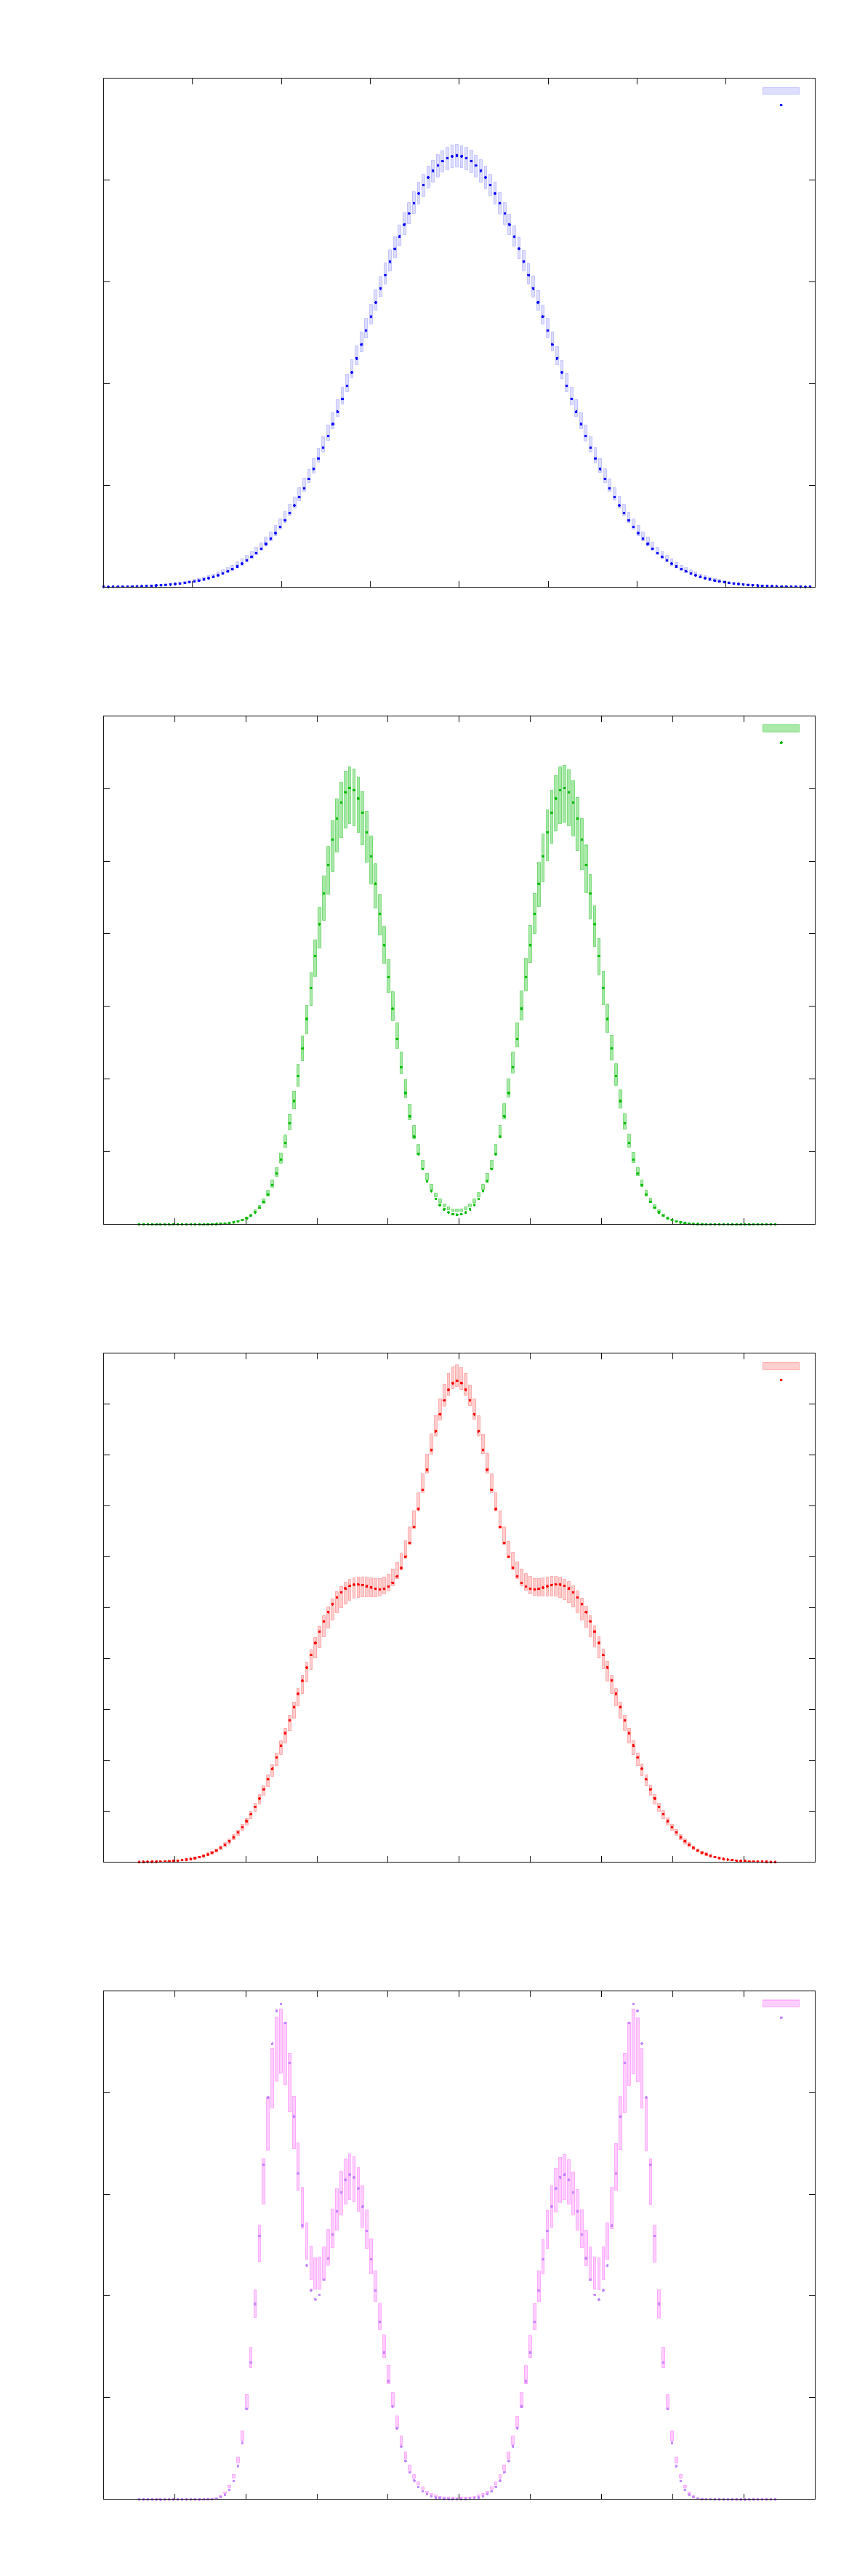
\includegraphics{plot-inc}}%
    \gplfronttext
  \end{picture}%
\endgroup
\end{document}
